The assignment was provided by Dr. Loveland as a Jupyter notebook. This notebook contained the code for generating the initial dataset. Empty cells were available for the three parts of the implementation.
In the first part we were to select a supervised learning method and train the model on the full dataset. I began this assignment by selecting the linear support vector classifier (SVC) as the supervised learning method. This method seemed like a good choice at the beginning. 
However, I ran into issue with the class-membership probability prediction. After some research, I was unable to determine the root cause of the issue. This led me to select a different supervised learning method.\par
At this point, I reviewed several classifiers available in scikit-learn [2]. I selected the random forest classifier as the supervised learning method. This method seemed like a good choice because it is an ensemble method that uses multiple decision trees to make predictions. 
Also, this method has been studied by others for use in co-training [3]. I was able to train the model on the full dataset, the two-point data set, and create a wrapper method for semi-supervised learning. The results of the predictions are shown in the results section.\par
If we inspect figure~\ref{fig:img0} we can see the entire dataset of twenty points. There are three classes of data points in this figure, these are called Class 1, Class 2, and unlabeled.

\begin{figure}[H]
    \centering
    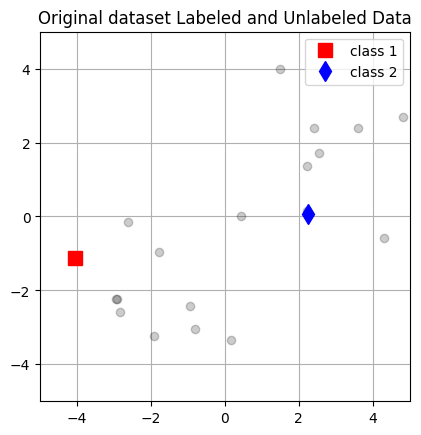
\includegraphics[width=0.5\textwidth]{images/img0.png}
    \caption{Initial Data Set}
    \label{fig:img0}
\end{figure}

